% Created 2021-01-06 śro 13:15
% Intended LaTeX compiler: pdflatex
\documentclass[11pt]{article}
\usepackage[utf8]{inputenc}
\usepackage[T1]{fontenc}
\usepackage{graphicx}
\usepackage{grffile}
\usepackage{longtable}
\usepackage{wrapfig}
\usepackage{rotating}
\usepackage[normalem]{ulem}
\usepackage{amsmath}
\usepackage{textcomp}
\usepackage{amssymb}
\usepackage{capt-of}
\usepackage{hyperref}
\renewcommand*{\contentsname}{Spis Treści}
\usepackage[margin=3cm]{geometry}
\hypersetup{colorlinks=true,linkcolor=blue}
\usepackage{fancyhdr}
\usepackage[yyyymmdd]{datetime}
\usepackage{graphicx}
\graphicspath{ {/home/thisconnect/pwsz/} }
\pagestyle{fancyplain}
\chead{Wyszukiwanie ścieżki datagramu w internecie}
\lhead{\includegraphics{pusb.png}}
\rhead{}
\cfoot{}
\lfoot{}
\rfoot{Patryk Kaniewski \linebreak GNU GPLv3}
\author{Patryk Kaniewski}
\date{\today}
\title{Wyszukiwanie ścieżki datagramu w internecie \\
Patryk Kaniewski}
\hypersetup{
 pdfauthor={Patryk Kaniewski},
 pdftitle={Wyszukiwanie ścieżki datagramu w internecie \\
Patryk Kaniewski},
 pdfkeywords={},
 pdfsubject={},
 pdfcreator={Emacs 27.1 (Org mode 9.3)}, 
 pdflang={Polish}}
\begin{document}

\begin{titlepage}
\begin{center}
{\Huge Wyszukiwanie ścieżki datagramu w internecie \par}
\vspace{2cm}
{\Large Patryk Kaniewski \par
}\vspace{2cm}
{\large 2021-01-06 }
\end{center}
\end{titlepage}
\setcounter{tocdepth}{2}
\tableofcontents \clearpage

\section{Grupa wykonująca zadanie}
\label{sec:org544e552}
\begin{itemize}
\item Patryk Kaniewski
\end{itemize}

\section{Wstęp}
\label{sec:orge9246f6}
\subsection{Cel ćwiczenia}
\label{sec:org4a05b4c}
Wyszukanie ścieżki datagramów w internecie
\subsection{Schemat ćwiczenia}
\label{sec:org22d4e51}
\begin{center}
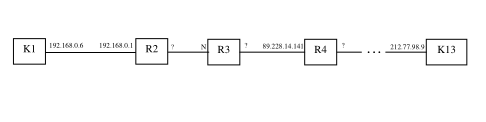
\includegraphics[width=.9\linewidth]{./schemat.png}
\end{center}
\subsection{Wymagany sprzęt}
\label{sec:org63bc0a9}
\begin{itemize}
\item Komputer z systemem POSIX
\end{itemize}

\subsection{Plan ćwiczenia}
\label{sec:orgf12c468}
\subsubsection{Część 1:}
\label{sec:org58ac94e}
\begin{enumerate}
\item Wyszukanie celu
\item Rejestracja ruchu ICMP
\item Znalezienie drogi
\end{enumerate}
\subsubsection{Część 2:}
\label{sec:orgb3e59e5}
\begin{enumerate}
\item Rejestracja ruchu ICMP i DNS
\item Znalezienie DNS i reverse DNS
\end{enumerate}
\subsubsection{Część 3:}
\label{sec:org85e9f9a}
\begin{enumerate}
\item Znalezienie drogi do dalekiego celu
\item Odczekanie ok. 30min
\item Znalezienie drogi do dalekiego celu
\item Porównanie dróg
\end{enumerate}


\section{Ćwiczenie}
\label{sec:orge11bf3e}
\subsection{Przed ćwiczeniem}
\label{sec:orgbc33336}
\subsubsection{Konfiguracja wstępna}
\label{sec:org3092bb9}
ip a show dev enp4s0
\begin{verbatim}
2: enp4s0: <BROADCAST,MULTICAST,UP,LOWER_UP> mtu 1500 qdisc fq_codel state UP group default qlen 1000
    link/ether b4:2e:99:e4:68:04 brd ff:ff:ff:ff:ff:ff
    inet 192.168.0.186/24 brd 192.168.0.255 scope global dynamic noprefixroute enp4s0
       valid_lft 32301sec preferred_lft 32301sec
\end{verbatim}
Wybranie celu oraz dalekiego celu (w tym ćwiczeniu \texttt{skierniewice.eu} oraz \texttt{theindependent.sg})
\subsection{Część 1}
\label{sec:orgcb6e7aa}
\subsubsection{Szukanie celu}
\label{sec:orga172832}
Wykonujemy ping do naszego celu
\begin{verbatim}
PING skierniewice.eu (94.152.194.219) 56(84) bytes of data.
64 bytes from 10.ires.pl (94.152.194.219): icmp_seq=1 ttl=55 time=6.41 ms
64 bytes from 10.ires.pl (94.152.194.219): icmp_seq=2 ttl=55 time=6.49 ms
64 bytes from 10.ires.pl (94.152.194.219): icmp_seq=3 ttl=55 time=6.43 ms
64 bytes from 10.ires.pl (94.152.194.219): icmp_seq=4 ttl=55 time=6.31 ms

--- skierniewice.eu ping statistics ---
4 packets transmitted, 4 received, 0% packet loss, time 3003ms
rtt min/avg/max/mdev = 6.310/6.412/6.492/0.065 ms

\end{verbatim}
\subsubsection{Rejestracja ruchu ICMP}
\label{sec:orga53b5c9}
Następnie używamy otrzymanego adresu IP do polecenia \texttt{traceroute -n -I 94.152.194.219} (opcja -n wyłącza odwracanie adresów ip na adresy domenowe; opcja -I wymusza używanie icmp echo do badania celow).


Rejestrujemy sesje za pomoca programu do przechwytywania pakietów np. wireshark i filtrujemy ICMP.
\begin{center}
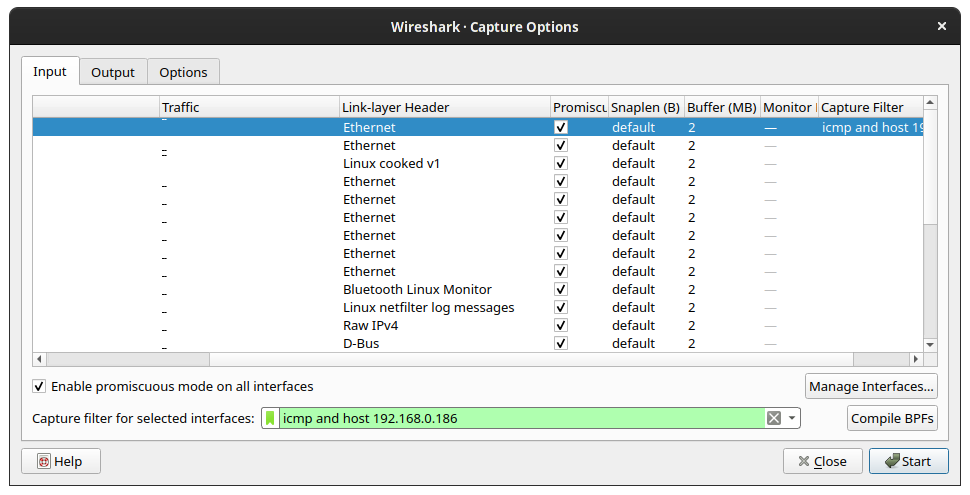
\includegraphics[width=.9\linewidth]{./part1/options.png}
\end{center}

\begin{verbatim}
traceroute to skierniewice.eu (94.152.194.219), 30 hops max, 60 byte packets
 1  192.168.0.1  0.223 ms  0.318 ms  0.473 ms
 2  91.214.0.129  1.167 ms  1.184 ms  1.200 ms
 3  * * *
 4  94.246.185.48  1.913 ms  1.960 ms  1.986 ms
 5  195.149.232.222  2.379 ms  2.431 ms  2.451 ms
 6  185.80.215.238  6.902 ms  6.804 ms  6.823 ms
 7  94.152.201.242  27.428 ms  26.699 ms  26.697 ms
 8  94.152.201.222  22.125 ms  21.498 ms  21.478 ms
 9  94.152.201.155  7.770 ms  7.394 ms  7.273 ms
10  94.152.194.219  6.205 ms  6.176 ms  6.286 ms
\end{verbatim}
\subsubsection{Wyniki}
\label{sec:org04591f3}
\begin{center}
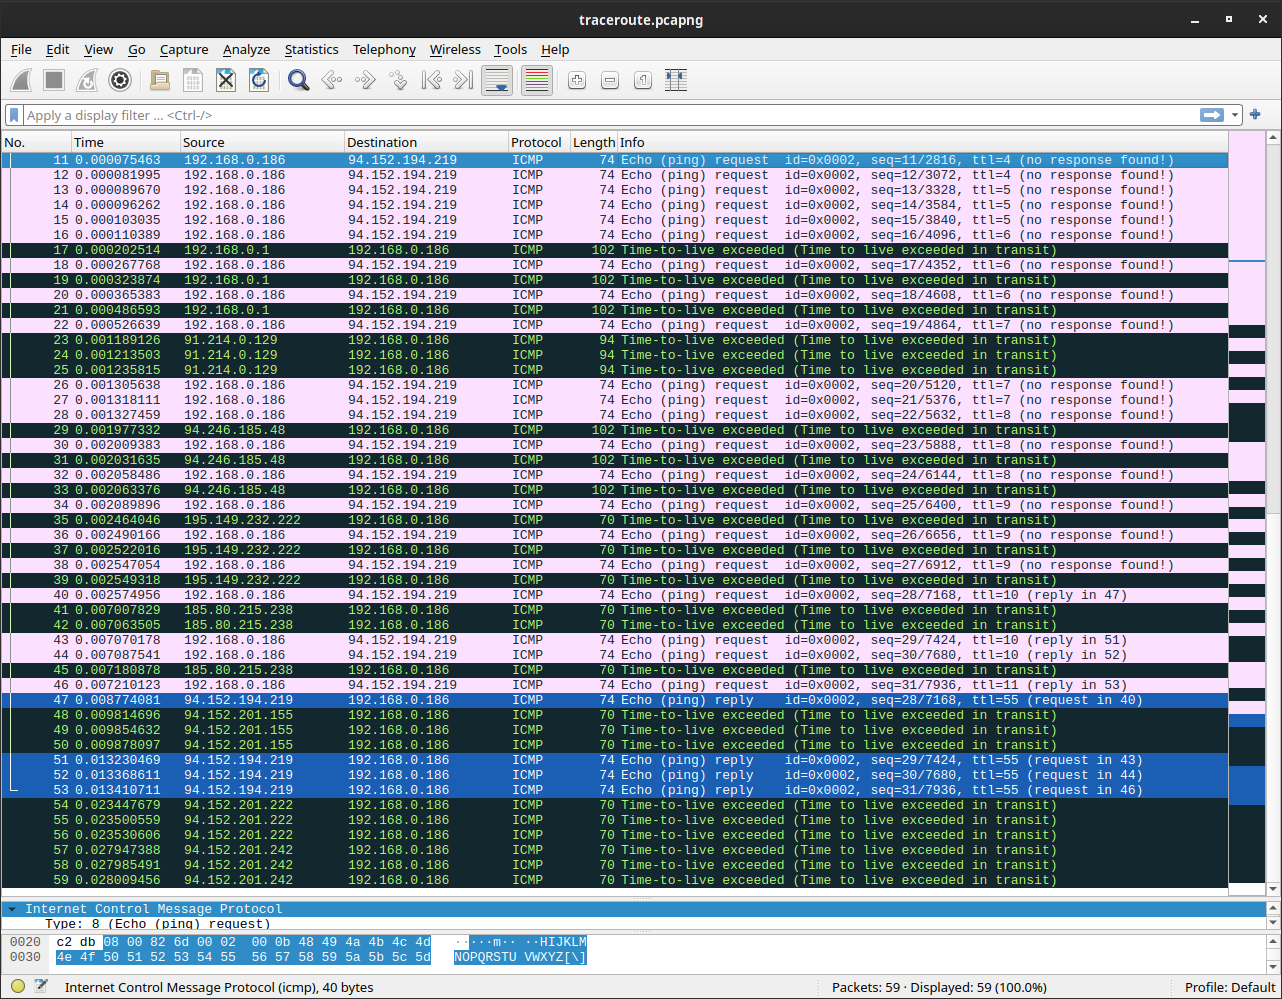
\includegraphics[width=.9\linewidth]{./part1/traceroute.png}
\end{center}
\begin{itemize}
\item Na różowo zaznaczone są Echo Request
\item Na czarno zaznaczone sa TTL exceeded
\item Na niebiesko zaznaczone sa Echo Reply
\end{itemize}

Nasza scieżka wyglada następująco:
\begin{center}
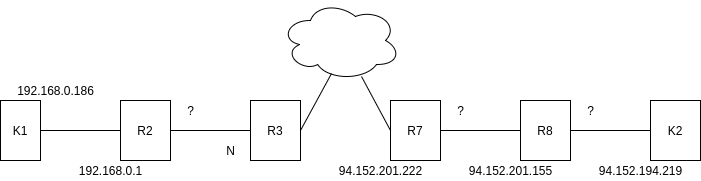
\includegraphics[width=.9\linewidth]{./part1/part1.png}
\end{center}

\subsection{Część 2}
\label{sec:org34cd84e}
\subsubsection{Rejestracja ICMP i DNS}
\label{sec:orgdbc4dd2}
W częsci drugie nieco zmieniamy nasze polecenie \texttt{traceroute -I skierniewice.eu} (opcja -I wymusza używanie icmp echo do badania celow).

Bez opcji -d, traceroute bedzie probował znaleść poprzez reverse DNS lookup adresy domenowe zwiazane z adresami ip.

Zmieniamy również opcje przechwytywania w programie przechwytywania pakietów (np. wireshark) na host K1.
\begin{center}
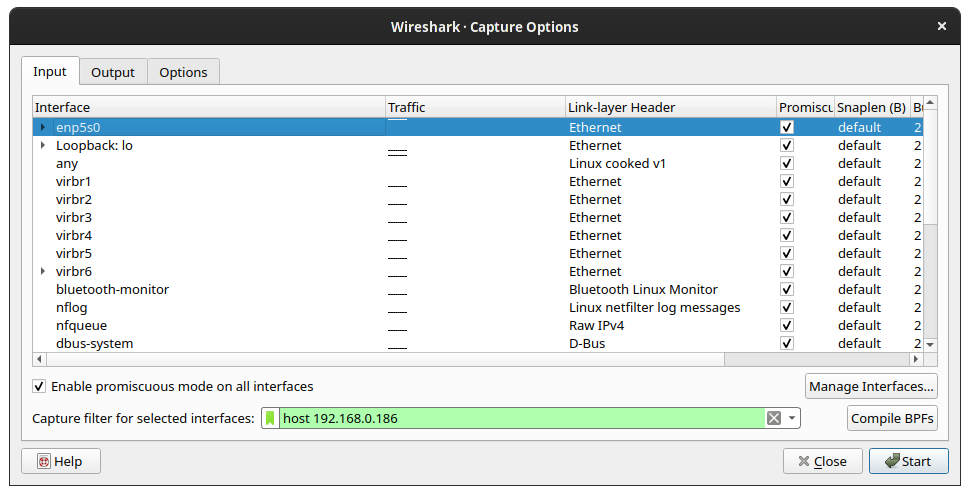
\includegraphics[width=.9\linewidth]{./part2/options.png}
\end{center}
\begin{verbatim}
traceroute to skierniewice.eu (94.152.194.219), 30 hops max, 60 byte packets
 1  _gateway (192.168.0.1)  0.247 ms  0.313 ms  0.481 ms
 2  91-214-0-129.timplus.net (91.214.0.129)  1.387 ms  1.379 ms  1.415 ms
 3  main-gw.timplus.net (91.214.0.1)  1.469 ms  1.490 ms  1.505 ms
 4  48.polmix2.epix.net.pl (94.246.185.48)  2.370 ms  2.397 ms  2.389 ms
 5  oxylion.tpix.pl (195.149.232.222)  2.654 ms  2.714 ms  2.739 ms
 6  185.80.215.238 (185.80.215.238)  7.172 ms  6.814 ms  6.805 ms
 7  5E98C9F2.static.tld.pl (94.152.201.242)  23.860 ms  21.250 ms  21.252 ms
 8  5E98C9DE.static.tld.pl (94.152.201.222)  25.080 ms  25.089 ms  25.100 ms
 9  5E98C99B.static.tld.pl (94.152.201.155)  14.678 ms  14.714 ms  14.730 ms
10  10.ires.pl (94.152.194.219)  6.568 ms  6.598 ms  6.619 ms
\end{verbatim}
\subsubsection{Wyniki}
\label{sec:org4634d97}
Aby ułatwić analizę packetdump możemy uzyć w wireshark display filter \texttt{icmp or dns}.
\begin{center}
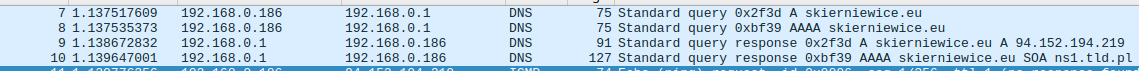
\includegraphics[width=.9\linewidth]{./part2/dnsA.png}
\end{center}
Pierwsze nasze zapytanie DNS jest typu A(AAA), aby przekonwertować nazwe domeny który przekazalismy traceroute (skierniewice.eu) na adres IPv4.
\begin{center}
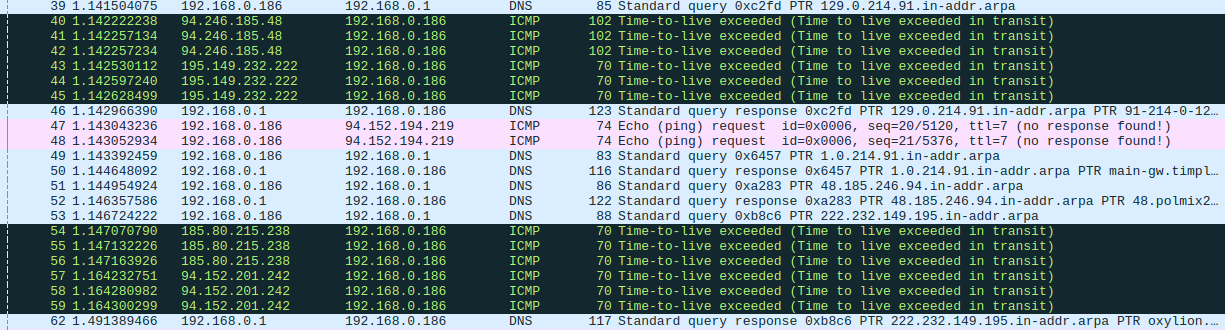
\includegraphics[width=.9\linewidth]{./part2/dnsPTR1.png}
\end{center}
Każde kolejne zapytanie bedzie typu PTR, aby przekonwertować adres IP na nazwe domeny. Warto zwrócić uwage na to że adres IP który został wysłany w zapytaniu PTR mial oktety odwrócone i \texttt{.in-addr.arpa} dodane na końcu.
\begin{center}
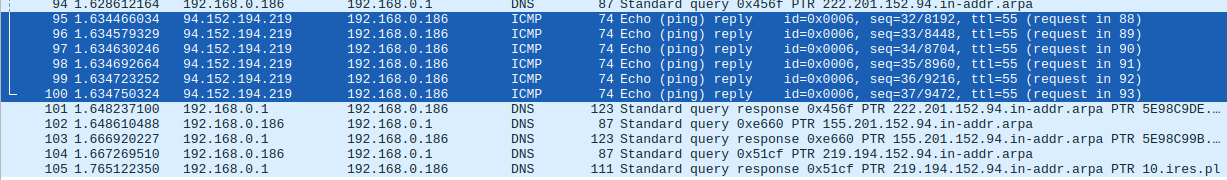
\includegraphics[width=.9\linewidth]{./part2/dnsPTR2.png}
\end{center}
Dokładnie tak samo wygląda zapytanie na ostateczny adres na który jest związany z domeną która testowaliśmy.
Ciekawym spostrzeżeniem może być że zapytanie PTR na ten sam adres który dostaliśmy z zapytania A \texttt{skierniewice.eu} ma inna nazwe domeny (\texttt{10.ires.pl}).

Można to zweryfikować za pomocą innych narzędzi (np. linux \texttt{dig} i \texttt{dig -x}).
\begin{verbatim}
;; QUESTION SECTION:
;skierniewice.eu.               IN      A

;; ANSWER SECTION:
skierniewice.eu.        3599    IN      A      
\end{verbatim}
\begin{verbatim}
;; QUESTION SECTION:
;219.194.152.94.in-addr.arpa.   IN      PTR

;; ANSWER SECTION:
219.194.152.94.in-addr.arpa. 3600 IN    PTR     10.ires.pl.
\end{verbatim}
\subsection{Część 3}
\label{sec:org292094d}
\subsubsection{Odległy cel}
\label{sec:org8213922}
Znalezienie odległego celu w dzisiejszych czasach może okazać sie problemem ze wzgledu na powszechność usług takich jak cloudflare, aws oferujacych wszelakie usługi proxy/cache.

Wybrano cel \texttt{theindependent.sg} znajdujący sie w azji południowo-wschodniej:
\begin{verbatim}
PING theindependent.sg (34.87.85.150) 56(84) bytes of data.
64 bytes from 150.85.87.34.bc.googleusercontent.com (34.87.85.150): icmp_seq=1 ttl=60 time=265 ms
64 bytes from 150.85.87.34.bc.googleusercontent.com (34.87.85.150): icmp_seq=2 ttl=60 time=266 ms
64 bytes from 150.85.87.34.bc.googleusercontent.com (34.87.85.150): icmp_seq=3 ttl=60 time=265 ms
64 bytes from 150.85.87.34.bc.googleusercontent.com (34.87.85.150): icmp_seq=4 ttl=60 time=265 ms

--- theindependent.sg ping statistics ---
4 packets transmitted, 4 received, 0% packet loss, time 3003ms
rtt min/avg/max/mdev = 265.312/265.624/266.329/0.410 ms
\end{verbatim}

Traceroute o godzinie 18:01.
\begin{verbatim}
traceroute to theindependent.sg (34.87.85.150), 30 hops max, 60 byte packets
 1  192.168.0.1  0.249 ms  0.352 ms  0.453 ms
 2  91.214.0.129  1.140 ms  1.146 ms  1.155 ms
 3  * * *
 4  94.246.185.48  1.893 ms  1.928 ms  2.005 ms
 5  195.149.233.101  2.436 ms  2.482 ms  2.673 ms
 6  188.47.253.245  2.565 ms  2.620 ms  2.547 ms
 7  * * *
 8  108.170.248.178  265.680 ms  265.580 ms  265.623 ms
 9  108.170.225.145  262.537 ms * *
10  209.85.243.180  263.452 ms  263.414 ms  263.415 ms
11  108.170.233.49  266.235 ms  265.706 ms  265.734 ms
12  * * *
13  * * *
14  * * *
15  * * *
16  * * *
17  * * *
18  * * *
19  * * *
20  * * *
21  34.87.85.150  265.372 ms  265.358 ms  265.202 ms
\end{verbatim}

\subsubsection{Ponowne szukanie drogi}
\label{sec:org43b1d4b}
Traceroute o godzinie 18:54.
\begin{verbatim}
traceroute to theindependent.sg (34.87.85.150), 30 hops max, 60 byte packets
 1  192.168.0.1  0.461 ms  0.415 ms  0.412 ms
 2  91.214.0.129  1.581 ms  1.587 ms  1.641 ms
 3  * * *
 4  94.246.185.48  2.100 ms  2.185 ms  2.193 ms
 5  195.149.233.101  2.670 ms  2.986 ms  2.674 ms
 6  188.47.253.245  3.412 ms  3.264 ms  3.483 ms
 7  108.170.248.195  265.707 ms 108.170.248.170  262.333 ms *
 8  108.170.248.203  263.531 ms 108.170.248.187  262.628 ms 108.170.248.171  261.930 ms
 9  108.170.229.13  264.222 ms 216.239.54.183  265.975 ms 108.170.225.191  269.693 ms
10  74.125.253.62  266.636 ms 74.125.37.250  260.637 ms 74.125.253.62  266.337 ms
11  66.249.95.195  265.662 ms 209.85.246.15  266.652 ms 66.249.95.195  265.467 ms
12  * * *
13  * * *
14  * * *
15  * * *
16  * * *
17  * * *
18  * * *
19  * * *
20  * * *
21  * * *
22  * * *
23  * * *
24  * * *
25  * * *
26  * * *
27  * * *
28  * * *
29  * * *
30  * * *
\end{verbatim}
\subsubsection{Różnice w drodze}
\label{sec:orgdc0a00e}
Aby porownać różnice można odrzucić pingi z traceroute za pomoca polecenia \texttt{awk '\{print \$1 "\textbackslash{}t" \$2\}' traceroute1.txt > trace1.txt} a następnie polecenia \texttt{diff} aby porównać te pliki.
\begin{verbatim}
4c4
< 3     91.214.0.1
---
> 3     *
8,12c8,12
< 7     108.170.248.170
< 8     108.170.248.194
< 9     108.170.225.145
< 10    72.14.233.235
< 11    172.253.68.225
---
> 7     108.170.248.195
> 8     108.170.248.203
> 9     108.170.229.13
> 10    74.125.253.62
> 11    66.249.95.195
\end{verbatim}
Widzimy dosyć duże zmiany w drodze(skok 7-11) oraz zmiane bramy u dostawcy internetu (skok 3 - timplus)




\section{Wnioski}
\label{sec:org3002bd9}
\subsection{Traceroute}
\label{sec:org25777b8}
Traceroute używa mechanizmu IP wartości TTL(czerwone) która jest obniżana za każdym razem kiedy pakiet jest przekierowany przez router. Router który obniża wartość TTL do 0, wysyła do source adress(niebieskie)  komunikat Time-to-live exceeeded in transit, za którego pomocą możemy poznać który router z jakim IP jest na skoku równym wysłanej wartości TTL.
\begin{center}
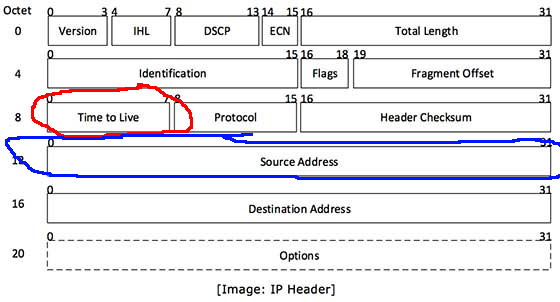
\includegraphics[width=.9\linewidth]{./ip_header.jpg}
\end{center}

\subsection{DNS}
\label{sec:orga89b315}
DNS jest systemem zamiany nazwy domen(przystępne dla człowieka) na adresy IP (używane w pakietach wysyłanych po sieci) oraz odwrotnie.
Zapytanie A zamienia domenę na adres IP, a zapytanie PTR zamienia adres IP na nazwę domeny. Zauważalne również była niezgodność w jednym przypadku pomiędzy zapytaniem odwrotnym a oryginalna nazwa domeny. Jest to spowodowane że jednostka odpowiedzialna za strefę .in-addr.arpa (w konketnym przypadku \texttt{10.ires.pl} (\url{https://www.ideo.pl/}) którzy tworzą i hostuja serwisy internetowe z ktorch \texttt{skierniewice.eu} korzysta) mogą być inne od tych ktorzy posiadają domenę (w konkretnym przypadku \texttt{skierniewice.eu})

\subsection{Routing}
\label{sec:org2c450e2}
W tym ćwiczeniu mogliśmy zaobserować mechanizm routingu dynamicznego. W części 3 zobaczyliśmy ze droga do naszego celu \texttt{theindependent.sg} została zmieniona w połowie. Bez dostępu do routerów nie możemy poznać przyczyny ale jest kilka najczęstszych przyczyn zmiany routingu:
\begin{itemize}
\item router na drodze miał awarie
\item została znaleziona szybsza droga (opóźnienie)
\item została znaleziona drożniejsza droga (przepustowość)
\end{itemize}

Najcześciej używanymi systemami routingu dynamicznego sa dla bram wewnetrznych(wewnątrz systemów autonomicznych np. sieć dostawcy internetu, firma):
\begin{itemize}
\item RIP - proste rozwiązanie na podstawie ilości skoków od x do y
\end{itemize}
\begin{itemize}
\item OSPF - złożone rozwiązanie oparte na stanie łącza (najczęsciej wiekszy priorytet dla połaczeń z wiekszą przepustowością)
\end{itemize}
Oraz dla bram zewnętrznych(połączenia pomiedzy systemami autonomicznymi np. pomiedzy dostawcami internetu, krajami, kontynentami):
\begin{itemize}
\item EGP
\item BGP
\end{itemize}

\subsection{Napotkane problemy}
\label{sec:org5bc164b}
\subsubsection{traceroute -I}
\label{sec:org78b39fb}
traceroute na systemie na ktorym przeprowadzane jest ćwiczenie (Archlinux) domyślnie nie używa ICMP echo (ping) do przeszukiwania drogi ze wzgledu na to że w dużej ilości sieci pakiety ICMP sa filtrowane
\begin{center}
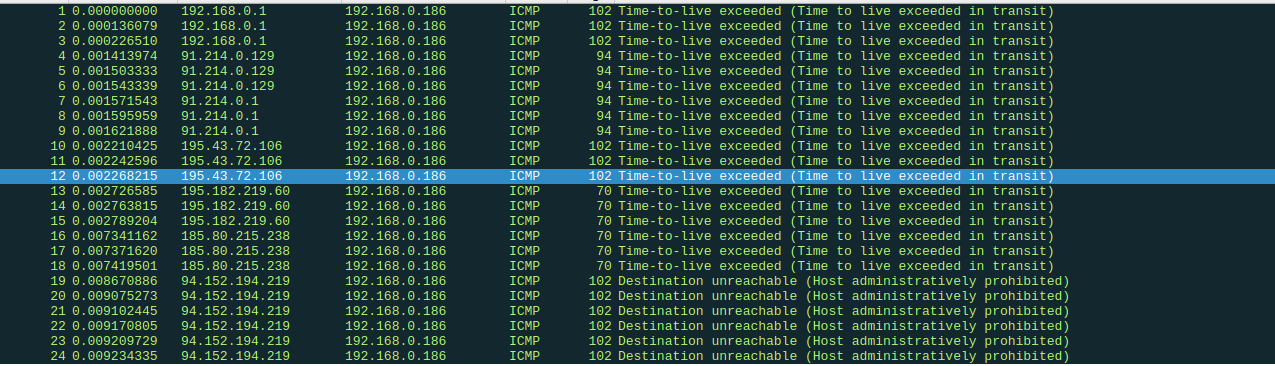
\includegraphics[width=.9\linewidth]{./problemy/problem1.png}
\end{center}

Rozwiązaniem tego było wyszukanie w manpage (\texttt{man traceroute}) o traceroute opcji -I która zmusza program do używania ICMP ping
\begin{center}
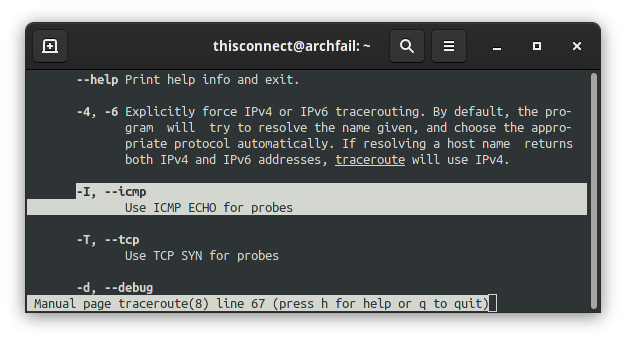
\includegraphics[width=.9\linewidth]{./problemy/rozwiazanie1.png}
\end{center}
\end{document}
